%!TEX root = document.tex

%%%%%%%%%%%%%%%%%%%%%%%%%%%%%%%%%%%%%%%%%%%%%%%%%%%%%%%%%%%%%%%%%%%%%%%%%%%
\begin{table}
\caption{Conditional entropy of various interactions (lower conditional
entropies are more informative).}
\label{table:ce_interaction}
\vspace{-2mm}
\centering
{\footnotesize
	\begin{tabular}{| >{\small}l | >{\small}r | }
		\hline
		\textbf{ Modality ($X$)} & $H(Y|X=true)$ \\
		\hline
		{ video } & 0.850 \\
		\hline
		{ link } & 0.915 \\
		\hline
		{ post } & 0.918 \\
		\hline
		{ photo } & 0.926 \\
		\hline
\multicolumn{2}{c}{}\\
		\hline
		\textbf{Action Type ($X$)}  & $H(Y|X=true)$ \\
		\hline
		{ tags }  &  0.920 \\
		\hline
		{ comments }  &  0.921 \\
		\hline
		{ likes }  &  0.924 \\
		\hline
\multicolumn{2}{c}{}\\
		\hline
		\textbf{ Direction ($X$) } & $H(Y|X=true)$ \\
		\hline
		{ outgoing }  &  0.928 \\
		\hline
		{ incoming }  &  0.935 \\
		\hline
\multicolumn{2}{c}{}\\
%	\end{tabular}
%\end{table*}
%%%%%%%%%%%%%%%%%%%%%%%%%%%%%%%%%%%%%%%%%%%%%%%%%%%%%%%%%%%%%%%%%%%%%%%%%%%
%	
%%%%%%%%%%%%%%%%%%%%%%%%%%%%%%%%%%%%%%%%%%%%%%%%%%%%%%%%%%%%%%%%%%%%%%%%%%%
%\begin{table*}
%	\begin{tabular}{| >{\small}l | >{\small}r |}
		\hline
		\textbf{Modality-Direction} ($X$) & $H(Y|X=true)$ \\
		\hline
		tags-outgoing & 0.885 \\
		likes-outgoing & 0.885 \\
		tags-incoming & 0.900 \\
		likes-incoming & 0.902 \\
		comments-outgoing & 0.908 \\
		comments-incoming & 0.912 \\
		\hline
%	\end{tabular}
\multicolumn{2}{c}{}\\
%	\begin{tabular}{| >{\small}l | >{\small}r |}
                \hline	
		\textbf{Action-Direction} ($X$) & $H(Y|X=true)$ \\
		\hline
		photo-outgoing & 0.857 \\
		video-outgoing & 0.863 \\
		link-outgoing & 0.895 \\
		link-incoming & 0.896 \\
		post-incoming & 0.902 \\
		post-outgoing & 0.906 \\
		video-incoming & 0.915 \\
		photo-incoming & 0.921 \\
		\hline
				
	\end{tabular}}
\end{table}
%%%%%%%%%%%%%%%%%%%%%%%%%%%%%%%%%%%%%%%%%%%%%%%%%%%%%%%%%%%%%%%%%%%%%%%%%%%

%%%%%%%%%%%%%%%%%%%%%%%%%%%%%%%%%%%%%%%%%%%%%%%%%%%%%%%%%%%%%%%%%%%%%%%%%%%
\begin{figure*}[tbp!]
\hspace{-15mm}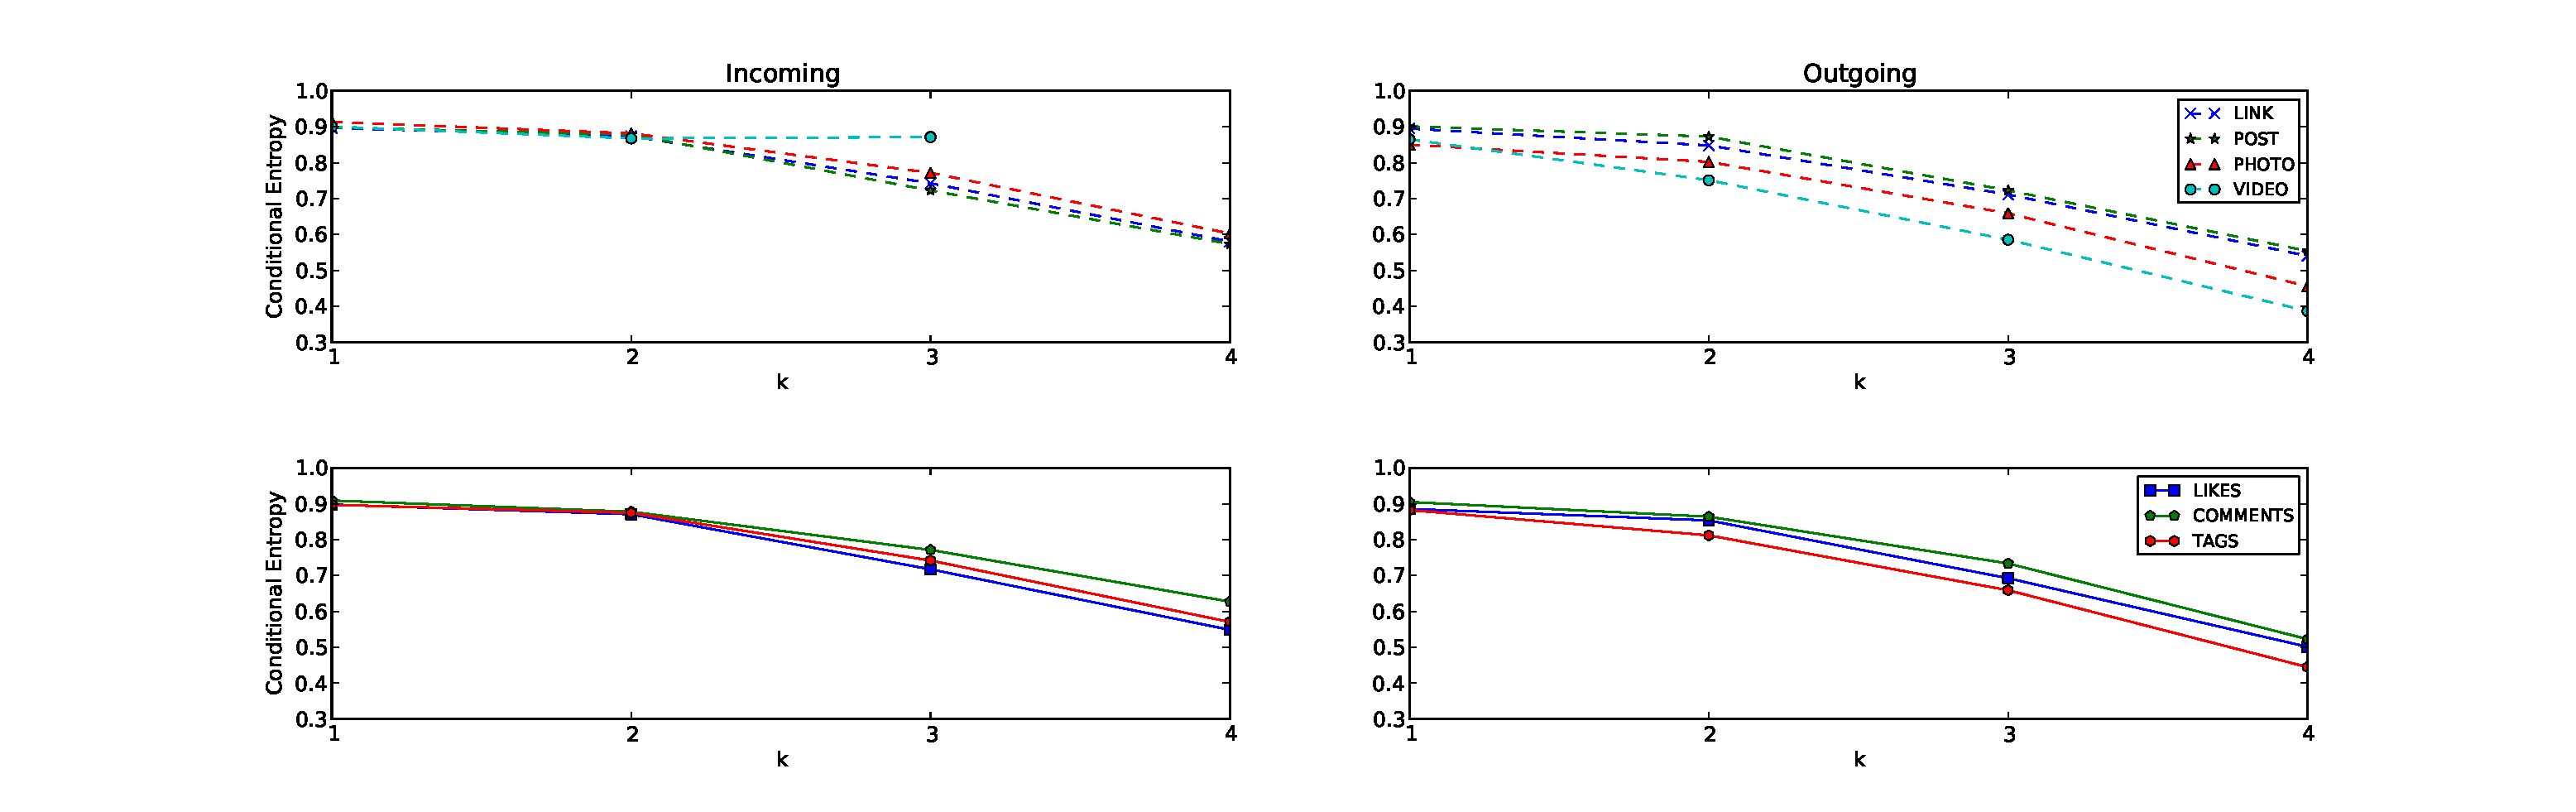
\includegraphics[width=210mm]{data/plots/vsk/ModalityActionsvsKFriends.eps}
\caption{Conditional Entropy  of modalities/activities for incoming/outgoing interactions vs item liked by at least k friends}
\label{Fig2}
\end{figure*}
%%%%%%%%%%%%%%%%%%%%%%%%%%%%%%%%%%%%%%%%%%%%%%%%%%%%%%%%%%%%%%%%%%%%%%%%%%%

In this section we analyze the informativeness of Interaction Social
Affinity Features (ISAFs), namely user interactions according to their
modality, type, and direction, as described in
Sec~\ref{sec:methodology}.

%namely those SAGs that are built w.r.t. a user $u$'s interactions.
A general method for measuring the amount of information that a 
feature $X^{u,i}_k$ provides w.r.t. predicting a user preference $\likes(u,i)$ (in this
case, just $\true$ or $\false$) is to calculate its conditional entropy:
\begin{align*}
H(\likes(u,i) &| X^{u,i}_k=\true)\\
& = -\sum_{y\in{(\true,\false)}} p(\likes(u,i)=y|X^{u,i}_k=\true) \ln( p(\likes(u,i)|X^{u,i}_k=\true))
\end{align*}
In general, a lower conditional entropy indicates a more informative
feature. Here we measure conditional entropy $H(\likes(u,i)| X^{u,i}_k=\true)$
rather than mutual information $I(\likes(u,i); X^{u,i}_k)$, as we found 
that mutual information is highly correlated with (and dominated by) the 
frequency of the feature $X^{u,i}_k=\true$ in the dataset.

%As defined in Sec~\ref{sec:methodology}, we have three distinctions for user
%interactions: modality, action, and directionality.  
First we analyze various interactions individually and jointly to understand what
interactions define SAGs with a high social affinity for a user $u$'s
preferences.  To this end, we make a few observations from the
conditional entropy analysis of Table~\ref{table:ce_interaction}:
\begin{itemize}
\item Interaction on {\em videos} seem to have a stronger preferential affinity 
than other modalities such as links, posts and photos.  This could be
  due to the fact that video viewing is time-consuming and users
  inherently only watch the videos of those whose preferences they
  often share.
\item Tagging has a slightly lower conditional entropy than
  commenting and liking, likely because the majority of tags contains 
  person name(s) on Facebook, indicating a direct social interaction. 
  % indicating that tagging.
\item A user is more likely to share preferences with someone who she
  initiates the interaction with (outgoing) vs. with someone who
  initiates the interaction with her (incoming).  As an extreme
  instance of this, we note that while outgoing photo and video
  interactions are most informative, it appears that incoming photo
  and video interactions are least informative.
\end{itemize}

In figure \ref{Fig2} we plot conditional entropy of modality and
action for incoming/outgoing interactions constrained to links
liked by at least $k$ friends in the SAG.  Figure \ref{Fig2} reiterates
many observations made above for various $k$.  In addition, we note that
preference affinity with a SAG increases as more people in the SAG
like the item --- then the more likely a user is to like an item.
While incoming interactions were not as predictive as outgoing
interactions for the same $k$, we note that higher $k$ for an incoming
interaction can be more predictive than lower $k$ for an outgoing
interaction.  Note that these graphs are cumulative in $k$, different from the 
exposure curve on exactly $k$ friends~\cite{Romero2011hashtag}. 
Our observations on user preference on items like by a number of Facebook friends 
suggest large cumulative number of friend interactions is more predictive 
-- this can be translated into recommender system design. 
Further investigation is needed to pinpoint whether or not there is 
diminishing returns on repeated exposures~\cite{ver2011stops,Romero2011hashtag} on $k$, 
and how this could be leveraged to design recommendation algorithms.
%We observed that 
%\begin{itemize}
%% NOTED ABOVE NOW
%  \item Some interactions are more predictive than other. For
%    eg. videos and photo interactions were found to be significantly
%    more predictive than post and link interactions. Similarly,
%    tagging action is often more predictive than commenting and
%    liking.
%  \item As noted by previous work~\cite{saez2011high}, we observe that
%    outgoing interactions are more predictive than incoming
%    interactions. Furthermore, the differentiation between
%    predictiveness modalities and actions is more pronounced in
%    outgoing interactions than in incoming interactions.
%  \item 

%This exhibits repeated exposure properties of epidemic
%models for social networks~\cite{Golub2010selectionbiase}.
%\end{itemize}


